\chapter{Background}\label{chap:background}

The background material in this chapter provides an overview of the theoretical concepts and fundamental technologies in which our deep learning approach is built. A few main concepts must be understood to appreciate the role of deep learning in data integration and predictive models. The first, and most fundamental to the discussion is an introduction to Artificial Neural Networks (ANNs), and their extension into the field of deep learning and information fusion. 

\section{Artificial Neural Networks}\label{sec:ann}
\subsubsection{Introduction}

Early attempts in designing computational systems to exhibit intelligent behaviour were conducted through formal rule-based programs referred to as Expert Systems~\cite{weiss1991computer}. In these systems, inference engines were used to apply a knowledge base of curated rules to deduce new rules and make predictions on future behaviour. It soon became evident that the sheer number of hard-coded rules required to simulate predictive behaviour was several orders of magnitude higher then capable to store or write for even moderately complicated tasks. This resulted in a shift from rigid and deductive systems towards inductive systems that learn to extract information from observed data. 

%Interesting and complex phenomenon (or behaviour) in nature are often fundamentally nonlinear  - can use this sentence to link expert systems to seeking solutions to nonlinear equations.
 
%Prior to the emergence of neural networks, 
Naturally, complex phenomena generally have dynamic correlations and nonlinear relationships. Accordingly, various techniques were developed to elucidate nonlinear relationships and emulate intelligent behaviour from observed training data. For instance, in statistics parametric models were developed so data could be described using finite-dimensional classes of nonlinear functions such as exponential, polynomial or power functions. However, these kinds of finite-dimensional models are limited in application to data adequately described by a bounded array of parametric functions. An additional approach, kernel methods, are based on non-linear projections of observed data into a latent space that can measure the distance between observations. New regression values or classifications are then predicted based on distances in the latent space. However, the construction of the kernel matrix in kernel-based methods becomes oppressive as the size of the data set increases, rendering these algorithms unfeasible for large data sets. Another class of models, ANNs, were discovered to elucidate many of the concerns of prior nonlinear models. ANNs thrive with large data sets and can learn to approximate any nonlinear function.

ANNs are loosely based on the function of biological neurons. In biology, neurons facilitate the flow of nerve impulses through networks that process and transmit information. The processing of inputs and outputs in neural structures allows biological neurons to adaptively learn and react based on previously observed patterns. ANNs implement this idea mathematically allowing them to act as nonlinear universal approximators. They perform this task by aggregating a cascade of simple nonlinear computations to form robust and complex nonlinear functions. Recently, ANNs have been particularly successful at solving large fundamental problems in natural language processing, voice recognition, and image classification~\cite{collobert2011natural, hinton2012deep, cirecsan2012multi}. 

\subsection{Mulitilayer Perceptron (MLP) Neural Networks}

The simplest form of an MLP is a feed forward and fully connected network with a single hidden layer, as shown in Figure \ref{fig:mlp}. A supervised learning problem for an MLP involves approximating a nonlinear function $f(x)$. The problem is considered supervised because each training example is associated with a label $y$. Consider data set $X \in \mathbb{R}^{m\times n} $ composed of m observations on n variables, where the $i$th observation is $x_i = (x_1,x_2,...,x_n)$. The computation in a single node of a neural network is simply the linear combination of vector $x_i$ with respective weights $\theta_i = (\theta_1,\theta_2,...,\theta_n)$ and an added bias term $b$:

    \begin{equation} \label{eq:lincomb}
        z = b + \sum_{i=1}^{n}  x_i \theta_i
    \end{equation}

The linear combination is then transformed by applying a nonlinear activation function $\psi(z)$, which maps the weighted inputs to the scalar output of the node. This simple computation within a single node is the basic building block of a MLP. MLPs contain at least two layers of these processing nodes (hidden and output layers), along with an input layer for training data. The hidden and output layers contain parallel processing nodes, each receiving input from the previous layer. This cascade of information from the input layer towards the output layer is why MLPs are classically defined as feed forward neural networks. 

\begin{figure}[h!]
    \centering
    \begin{subfigure}[b]{0.59\textwidth}
        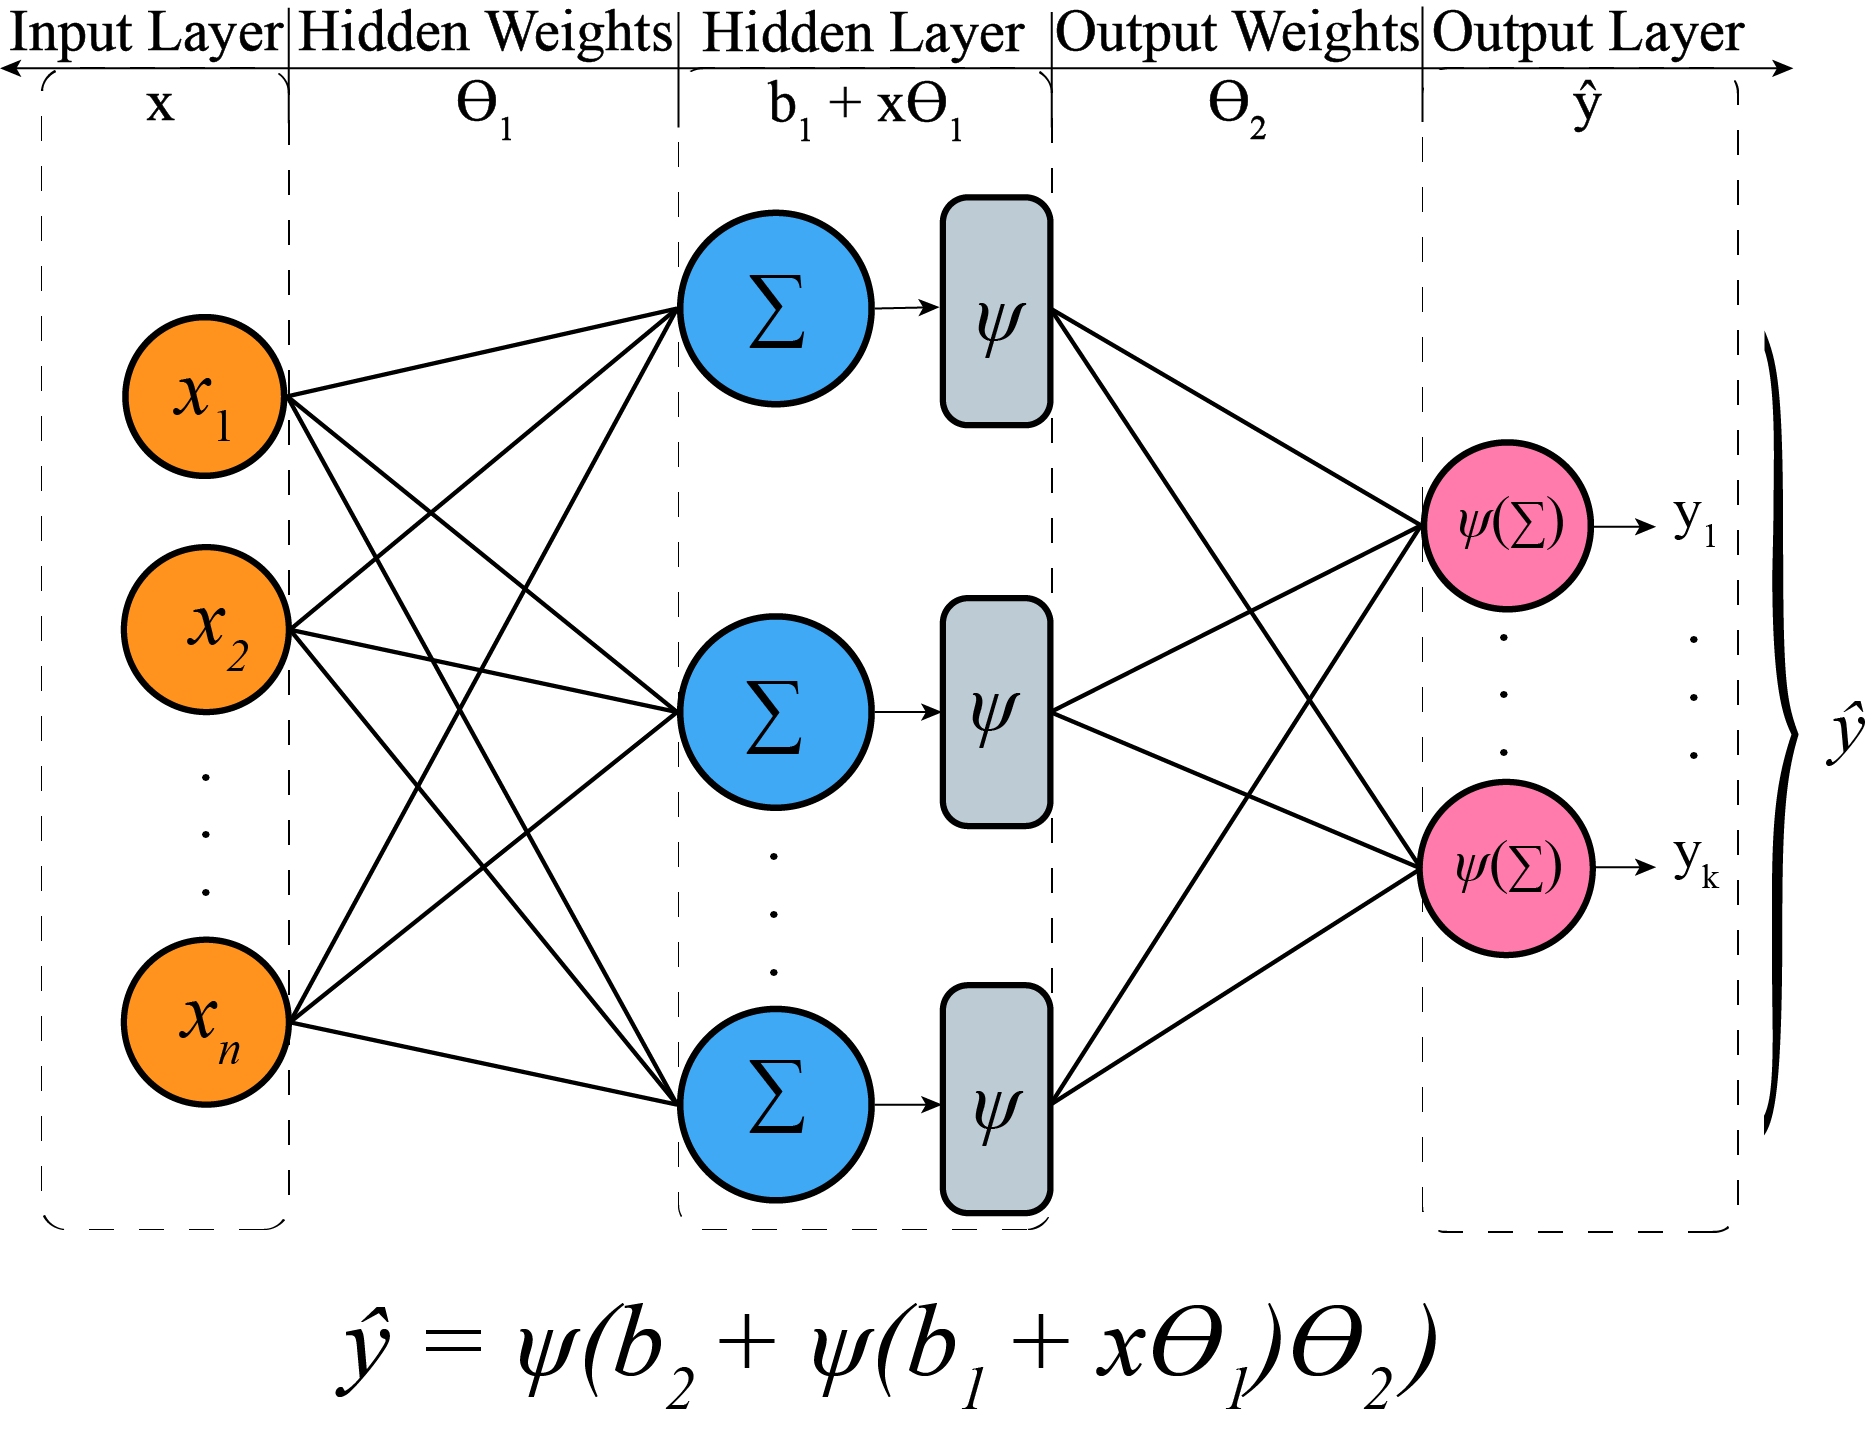
\includegraphics[height = 6cm, width=\textwidth]{img/mlp.png}
        \caption{Feed Forward Multilayer Perceptron}
        \label{fig:mlp}
    \end{subfigure}
    \hfill
    \begin{subfigure}[b]{0.40\textwidth}
        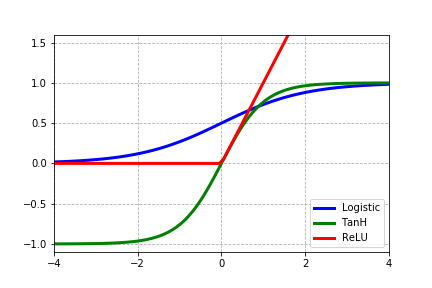
\includegraphics[height = 6cm, width=\textwidth]{img/actfunc.png}
        \caption{Common Activation Functions, $\psi$}
        \label{fig:actfunc}
    \end{subfigure}
    \caption{\ref{fig:mlp}) Structure of a feed forward MLP with three layers. \ref{fig:actfunc}) The output for Logistic, Tanh and ReLU activation functions for input value range [-4,4].}\label{fig:mlp_actfunc}
\end{figure}
% Change the italics brackets to regular 
% Add activation function to hidden layer 
%Define supervised classification and regression before hand

A nonlinear activation function $\psi$ allows the composititional output function $ \hat{y}$ to map inputs non-linearly to outputs (reference). Deeper MLPs will contain many more hidden layers then displayed in Figure \ref{fig:mlp}, and a neural network with $n$ layers can be defined recursively as:
\begin{equation}
        \hat{y} = \psi(\theta_{n}(\psi(\theta_{n-1}(\psi(\theta_{n-2}(\ldots \psi(\theta_{1} x + b_{1}) \ldots)) + b_{n-2})) + b_{n-1}) + b_{n}) 
\end{equation}

Where the structure of $\hat{y}$ depends on the desired task (e.g nonlinear regression or classification). For regression problems, $\hat{y}$ is a real value, and for classification problems, $\hat{y}$ is a $k$ dimensional vector of real values. So although it is generally advantageous for hidden units to have nonlinear activation functions, the choice of activation functions for output layers will largely depend on the desired task. For nonlinear regression, a linear activation function is generally adequate. However, in classification problems, it can be useful to view the $k$ dimensional output vector $\hat{y} = (y_1,y_2,..., y_k)$ as providing the probabilities a given input example resides in each respective class. This produces a probability distribution over the $k$ classes, where entries fall between $(0,1)$, and the sum of vector $\hat{y}$ is one. This behaviour is accomplished by the softmax function:
\begin{equation}
       softmax(z) =  \frac{e^{z_j}}{\sum_{i=1}^{k}e^{z_i}} \;\;\; \mbox{for} \;\;\; j = 1,\ldots,k
\end{equation}

Where $softmax(z)$ represents the categorical distribution of arbitrary $k$ dimensional vector $z$. Furthermore, with a formally defined arbitrary output function $\hat{y}$, the next step requires the artificial neural network to learn weights and biases in order to produce desired outputs given input data.

\subsubsection{The Cost Function}
Training an artificial neural network relies on determining the network parameters that minimize the error between outputs $\hat{y}$ and true values $y$. This entails producing a model function, that given inputs, can produce the output to the closest degree. In machine learning, the notion of a good model is explicitly defined using some cost function $J(\hat{y},y;\Theta)$, where $\Theta = \{\theta, b\}$ is the set of all network weights and biases. The cost function keeps track of the models prediction error, and finding better models equates to finding better network parameters that minimizes the cost function. For nonlinear regression, a commonly used measure of cost is simply the mean squared error between the output of the neural network and the true values:
\begin{equation} \label{eq:mse} 
    J(\hat{y},y;\Theta) = \sum_{i=1}^{m}(y_i - \hat{y_i})^{2}
\end{equation}

For classification problems, it is often beneficial to represent categorical true labels $y$ as binary vectors. This is referred to as a one hot encoding, where the $i$th position of class $i$ is one, and every other term is zero. For example, in a five class problem, a class of three would be coded as $y = [0,0,1,0,0]$. In this way, error must be calculated for each potential class $k$ over all examples in the sample set. Accordingly, the most commonly used cost function for classification problems is the cross entropy loss:
\begin{equation} \label{eq:softmax}
    J(\hat{y}, y; \Theta) = - \frac{1}{m}\sum_{i = 1}^{m}\sum_{j = 1}^{k} \lbrack y_{i,j} \log(\hat{y_{i,j}}) + (1 - y_{i,j})\log(1 - \hat{y_{i,j}}) \rbrack
\end{equation}

In the computation of cross-entropy loss, $k$ error terms are generated for every training example. The cross-entropy loss represents the log probability of classes given the model - that is, maximizing the likely hood of a training example belonging to a specific class is equivalent to minimizing the cross entropy loss between $\hat{y}$ and $y$. 

\subsubsection{The Optimization Algorithm}
The cost, $J(\hat{y}, y; \Theta)$, is conveniently a function of the training examples and model parameters $\Theta$. In order to efficiently minimize the cost function, it is useful to observe how the cost changes with respect to weights $\theta$. Formally, this is expressed with the partial derivative $\frac{\partial J}{\partial \theta}$. With this expression, we can search for weights in the direction that cost $J$ decreases. This technique, called gradient descent, minimizes cost by iteratively updating $\theta$ in the opposite direction of the gradient:
\begin{equation}
    \theta_j = \theta_j - \alpha \frac{\partial}{\partial \theta_j} J(\hat{y},y;\Theta) \;\;\; \mbox{for} \;\;\; j = 1,\ldots,n
\end{equation}

%Other optimization techniques have been developed, but not many of them are shown to generalize performance, andrew ng (gradient descent/adam), an exception is the adam optimizer (reference)  

Where $\alpha$, the learning rate, controls the size of steps made in the direction of the negative gradient. Furthermore, in order to compute the gradients of the cost with respect to model weights, an algorithm called backpropogation is commonly used. The cost function, as one large nested composite function, contains all of the computations in the neural network. With this, the backpropagation algorithm cleverly applies the chain rule of calculus to recursively compute the gradients of each weight with respect to the outputs so weights can be updated incrementally using gradient descent. 

\begin{figure}[h!]
    \centering
    
    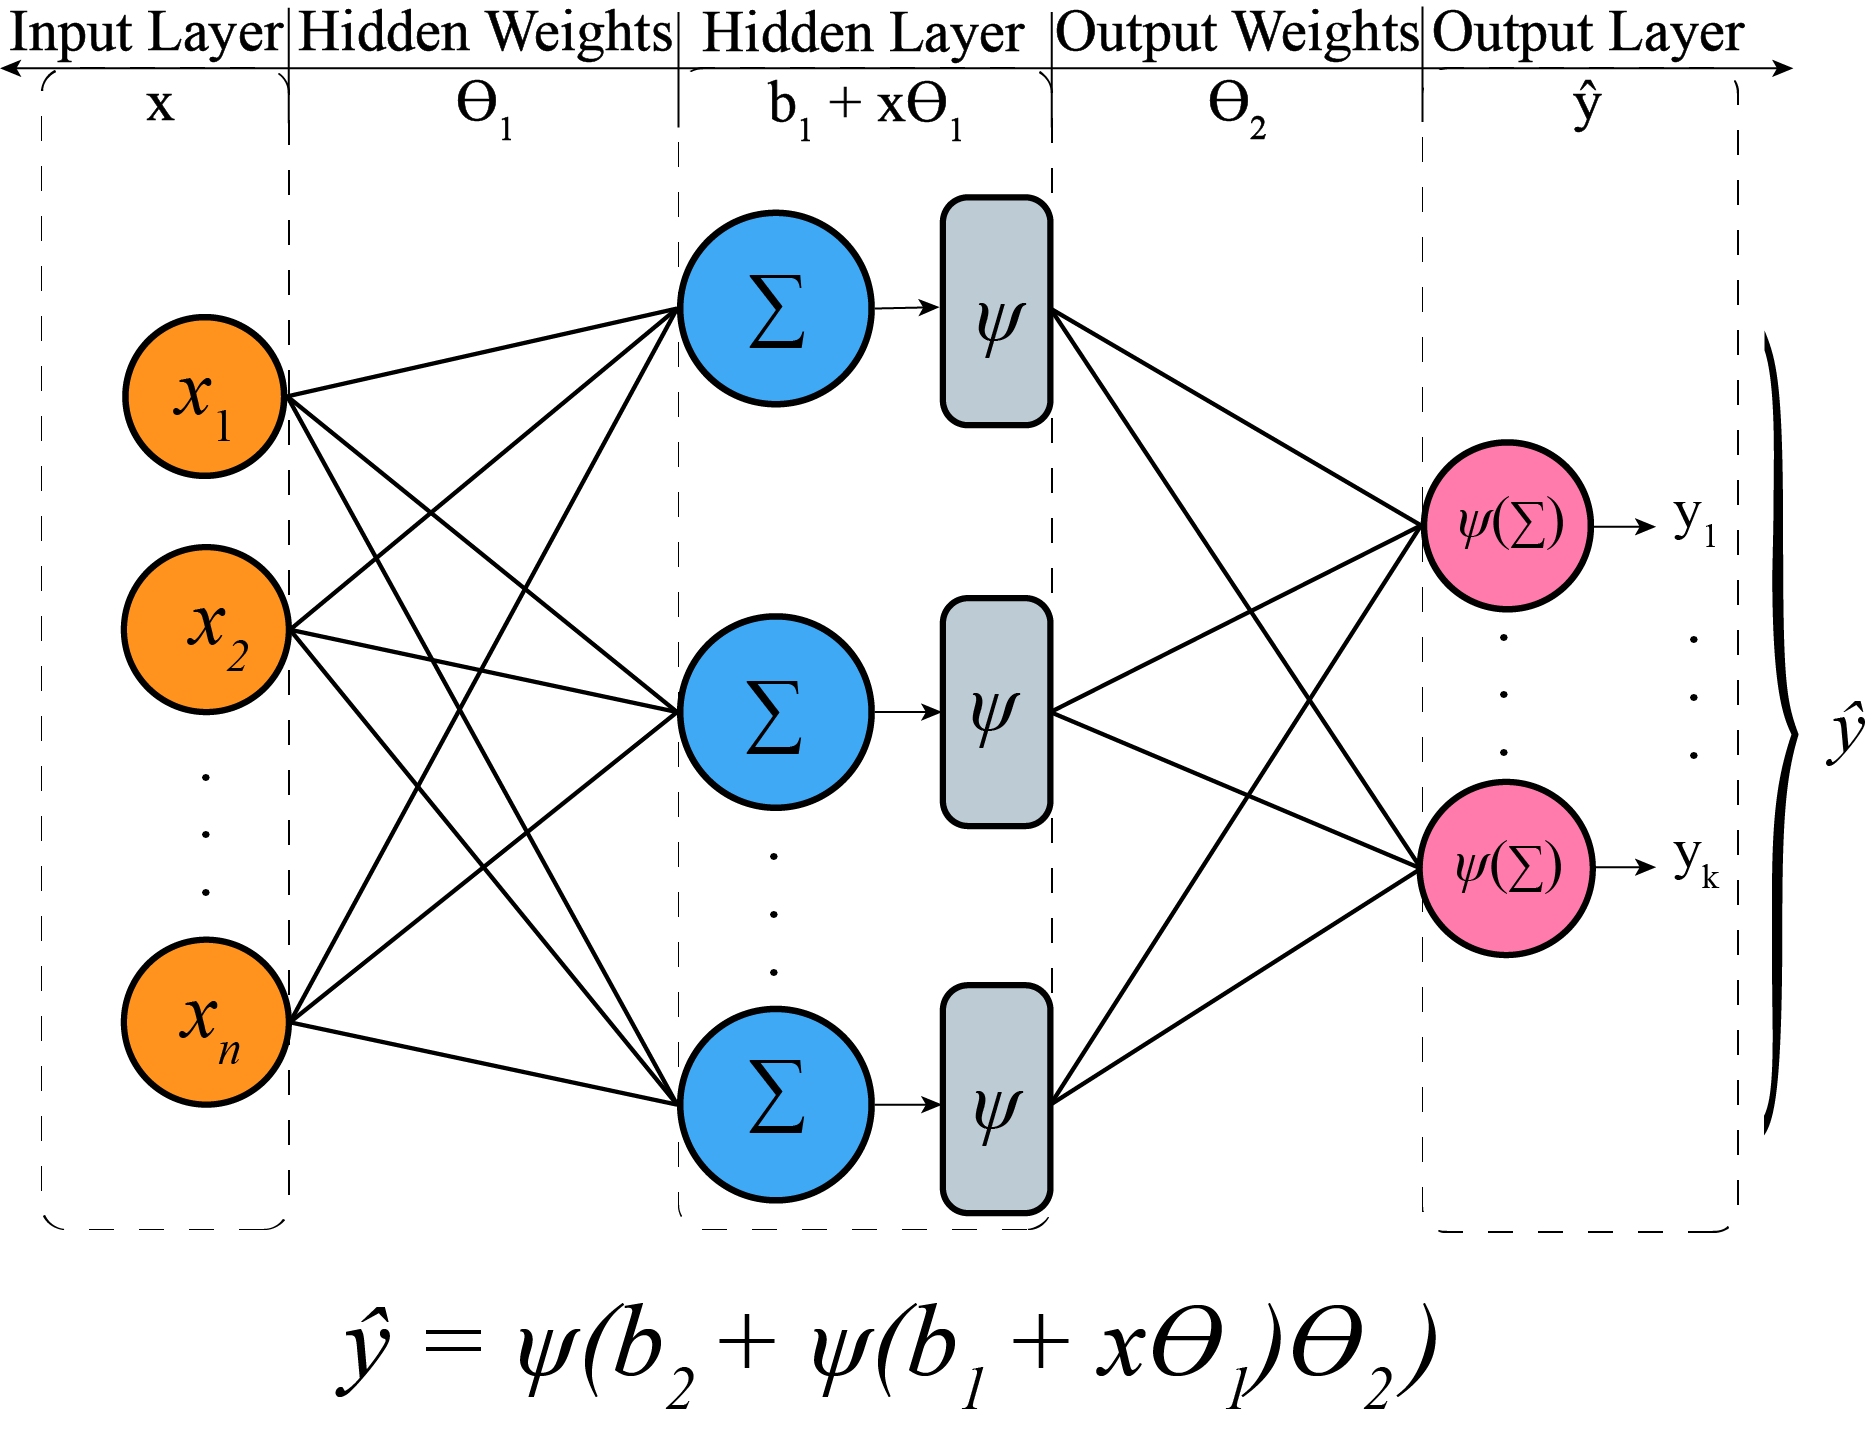
\includegraphics[height = 6cm, width=\textwidth]{img/mlp.png}
    \caption{Feed Forward Multilayer Perceptron}
    \label{fig:mlp}
    \caption{\ref{fig:mlp}) Structure of a feed forward MLP with three layers. \ref{fig:actfunc}) The output for Logistic, Tanh and ReLU activation functions for input value range [-4,4].}\label{fig:mlp_actfunc}
\end{figure}

%Should I go through an algorithmic overview of this process?
%Or a demonstration with a model neural network?

%Deeper neural networks simply continue to stack these operations 



%In Figure \ref{fig:actfunc}, we see that the tanh and logistic functions have sigmoidal shapes, mapping all inputs between $(-1,1)$ and $(0,1)$, respectively. In the output layer, this kind of behaviour makes them useful for classification problems. Though for nonlinear regression, a linear output activation would be beneficial. Accordingly, the choice of activation functions will largely depend on the desired task, but it is generally desired for the hidden units to have nonlinear activation functions. Deeper MLPs will contain many more hidden layers then displayed in Figure \ref{fig:mlp}, 

%%The cost function, as one large nested composite function, contains all of the computations in the neural network. 

\subsection{Stacked Denoising Autoencoders}

%This continues to the stacked denoising variant

